\documentclass{article}
\usepackage{amsmath}
\usepackage{graphicx} % Load the graphicx package
\usepackage{xcolor} % For color support
\usepackage{fancyhdr} % For custom headers and footers
\usepackage{titling} % For customizing the title layout
\usepackage{indentfirst}
\usepackage[margin=1in]{geometry} % Set margins

\title{\textcolor{black}{\Huge\bfseries Trabalho de Redes Neurais Artificiais}\\[100pt]
{\huge\bfseries Poda Aleatória de ELMs e regularização.}} % Highlighted title

\author{\\[50pt]{\bfseries Aluno : Arthur Felipe Reis Souza.} \\[50pt]
{\bfseries Professor : Antonio de Padua Braga.} \\[ 50pt]}

\date{\today}

% Custom header and footer
\pagestyle{fancy}
\fancyhf{} % Clear default header and footer
\fancyfoot[C]{\thepage} % Page number in the center of the footer
\renewcommand{\headrulewidth}{0pt} % Remove header rule



\begin{document}

\maketitle % Creating the title.

\newpage

\pagestyle{fancy} % Define estilo de página como fancy

\section*{\\[50pt] Sumário}

\subsection*{\\[30pt] Introdução}
\begin{itemize}
    \item Introduzir as Redes Neurais Artificias.
    \item Explicar a função de custo multiobjetiva, e a necessidade da regularização.
\end{itemize}

\subsection*{\\[30pt] Desenvolvimento}
\begin{itemize}
    \item Explicar as redes neurais ELM (Extreme Learning Machine).
    \item Explicar os métodos de regularização que serão usados.
    \item Funções de treinamento com os metodos de regularização.
\end{itemize}

\subsection*{\\[30pt] Resultados e Discussões}
\begin{itemize}
    \item Aplicar esses métodos de regularização nos datasets.
    \item Variar os hiperparâmetros e analisar os resultados.
    \item Discutir os resultados para a variação dos hiperparâmetros.
\end{itemize}

\subsection*{\\[30pt] Conclusão}
\begin{itemize}
    \item Realizar conclusões sobre as análises feitas no trabalho.
\end{itemize}

\subsection*{\\[30pt] Referências}
\begin{itemize}
    \item Referências bibliográficas utilizadas no trabalho.
\end{itemize}

\newpage






\section*{Introdução}

\vspace{15pt}

Atualmente, com a evolução tecnológica e o desenvolvimento em áreas da ciência e engenharia, é possível evidenciar pessoas e objetos gerando dados o tempo inteiro. Os algoritmos de Machine Learning são modelos estatísticos e matemáticos que, quando implementados em 1 computador, se tornam úteis para extrair informações relevantes acerca dessa grande quantidade de dados. A escolha do algoritmo de Machine Learning dependerá do tipo de problema a ser resolvido, também da complexidade e tamanho da base de dados. Algoritmos diferentes podem ter um desempenho semelhante, mesmo para uma grande diferença de tempo e recurso computacional gasto. Portanto, é necessário analisar profundamente o desempenho de cada algoritmo para um mesmo problema, e escolher o que terá um melhor equilíbrio entre custo e performance[3].



\vspace{15pt}


\begin{figure}[h]

    \centering
    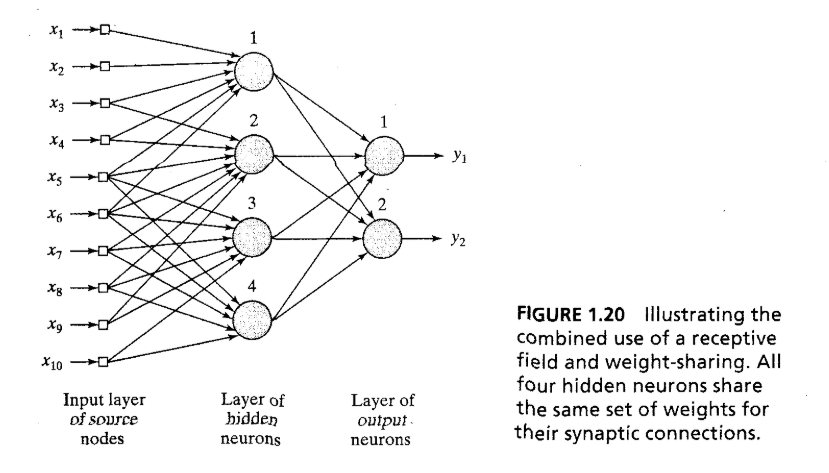
\includegraphics[height=3in]{neural_net_pic.png}
    \caption{Imagem retirada do livro Neural Networks, Simon Haykin.[1]}
    \label{fig:example}

\end{figure}


\vspace{15pt}

As Redes Neurais Artificias são algoritmos de Machine Learning que consistem no ajuste dos parâmetros da rede para minimizar, parcialmente ou totalmente, uma função de custo J. Foi aprendido na fase inicial do curso a minimização de uma função de custo J que tem caráter uniobjetivo. Para isso, se ajustava os parâmetros da rede de forma a minimizar o erro de saída da rede, aproximando a saída da rede à saída desejada. O problema de minimizar apenas o erro de saída da rede é que, quando o modelo é muito complexo ele tenderá ao overfitting, que acontece quando a rede não aprende corretamente a função geradora dos dados e gera saídas incorretas para os dados de teste. As técnicas de regularização surgem para controlar a complexidade do modelo, e tendem a evitar esse overfitting. No trabalho serão estudadas as técnicas de regularização Ridge Regression (L2 Regression) e o Pruning para as Redes Neurais do Tipo ELM (Extreme Learning Machines). Serão utilizadas bases de dados que contém problemas de classificação e regressão, onde os resultados serão analisados. Com essa análise, uma Conclusão sobre esses métodos de regularização será feita.


\newpage


\section*{Metodologia}

No trabalho, foi utilizada as redes neurais ELM (Extreme Learning Machine). As redes neurais ELM (Extreme Learning Machine) tem uma estrutura parecida com as redes do tipo MLP (Multi Layer Perceptron), onde as entradas são transformadas até a camada de saída. No entanto, elas se diferem na forma como são treinadas. As redes ELM se baseiam no Teorema de Cover, o qual afirma que uma expansão aleatória de alta dimensão da camada intermediária resulta em uma chance alta de linearização do problema. Sendo assim, com o problema linearmente separável na camada de saída basta aplicar um modelo linear que melhor irá se adequar ao problema.[4]

\vspace{15pt}

Após a criação das redes neurais ELM, métodos e heurísticas foram usadas no fito de tentar regularizar o modelo. Afim de encontrar os parâmetros que resultam em um melhor desempenho do modelo, foi utilizada a técnica Grid Search Cross-Validation. O Grid Search Cross-Validation é um algoritmo utilizado para encontrar os parâmetros que resultam em um melhor desempenho do modelo. Para isso, cria-se um grid com todas as possibilidades possíveis que os parâmetros podem assumir, em seguida, testa-se cada uma das configurações com o algoritmo Cross-Validation. Há maneiras diferentes de implementar o Cross-Validation, no trabalho foi usado o K-fold Cross-Validation.

\vspace{15pt}

O K-fold Cross-Validation é um algoritmo utilizado para treinar e testar o modelo. Ele se baseia em dividir os dados de entrada em K grupos. Dentro desses K grupos, (K - 1) serão utilizados para treino e 1 grupo para teste. Esse processo se repete até que todos os K grupos tenham sido usados para treino e teste, e ao final a média do desempenho será utilizada para avaliar o modelo com relação a uma métrica específica. Para os problemas de classificação, a métrica utilizada será a acurácia. Para os problemas de regressão será o MSE (erro quadrático médio).

\vspace{15pt}

\begin{figure}[h]

    \centering
    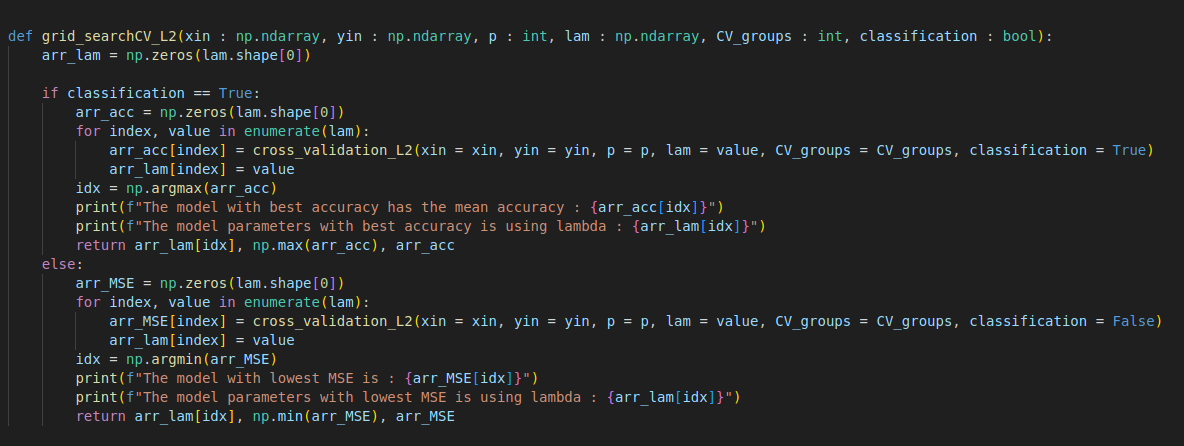
\includegraphics[height=2.5in]{grid_search_L2.png}
    \caption{Código do Grid-Search para regularização Ridge Regression.}
    \label{fig:example}
    
\end{figure}


\vspace{15pt}

Além das heurísticas propostas no enunciado do trabalho (Ridge Regression e o Random Pruning), também foi utilizada a heurística de eliminação dos pesos com menos relevância e influência na saída do modelo. Para a análise do modelo, 6 bases de dados foram escolhidas de forma a visualizar bem a generalização do mesmo. 3 dessas bases são de regressão e 3 de classificação. As bases de dados de classificação são : base de dados Xor, base de dados Circle e o Breast Cancer. As bases de dados de regressão são : Função senoidal, Boston House e Wine Quality. Todas as bases que não foram geradas internamente em python foram extraídas do site de competição Kaggle.

\newpage

\subsection*{Ridge Regression}

\vspace{15pt}

O método de regularização Ridge Regression consiste em adicionar um termo de penalização na função de custo. Esse termo de penalização tem por objetivo limitar a magnitude dos pesos w e por consequência evitar o modelo do overfitting.

\vspace{15pt}

\begin{figure}[h]

    \centering
    
\includegraphics[height=0.5in]{funcao_custo_pen.png}
    \caption{Função de custo adicionada do termo penalizador.[4]}
    \label{fig:example}
    
\end{figure}

\vspace{15pt}

Agora, a função de custo é multiobjetiva, pois envolve duas funções objetivos com um comportamento conflitante. Ou seja, ao minimizar uma das funções objetivos não minimiza a outra em conjunto. Para encontrar os parâmetros w que minimizam essa função de custo multiobjetiva, basta-se calcular a derivada dessa função de custo em relação aos parâmetros.

\vspace{15pt}

\begin{figure}[h]

    \centering
    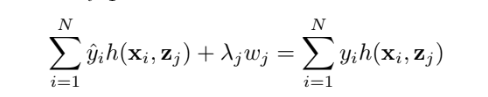
\includegraphics[height=0.5in]{rel_funcao_multi.png}
    \caption{Equação que resulta na minimização da função de custo multiobjetiva.[4]}
    \label{fig:example}
    
\end{figure}

\vspace{15pt}

A equação acima mostra a minimização para uma dimensão caracterizada por wj. Para abranger todos os parâmetros w que serão ajustados, o problema será mostrado como um conjunto de equações lineares, e resolvido através da álgebra linear.


\vspace{15pt}

\begin{figure}[h]

    \centering
    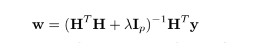
\includegraphics[height=0.35in]{pen_al.png}
    \caption{Regularização descrita por uma relação de álgebra linear.[4]}
    \label{fig:example}
    
\end{figure}

\vspace{15pt}

O termo penalizador pode ser decidido seguindo diferentes heurísticas. Cada heurística diferente tem como objetivo somar um termo no cálculo da pseudoinversa. Esse termo penalizador também é útil para evitar a existência de matrizes singulares. No desenvolvimento do trabalho, a matriz de parâmetros W estava explodindo para valores muito altos, esse problema foi resolvido com a utilização de um termo penalizador na matriz H que gerou a pseudoinversa.

\vspace{15pt}

\begin{figure}[h]

    \centering
    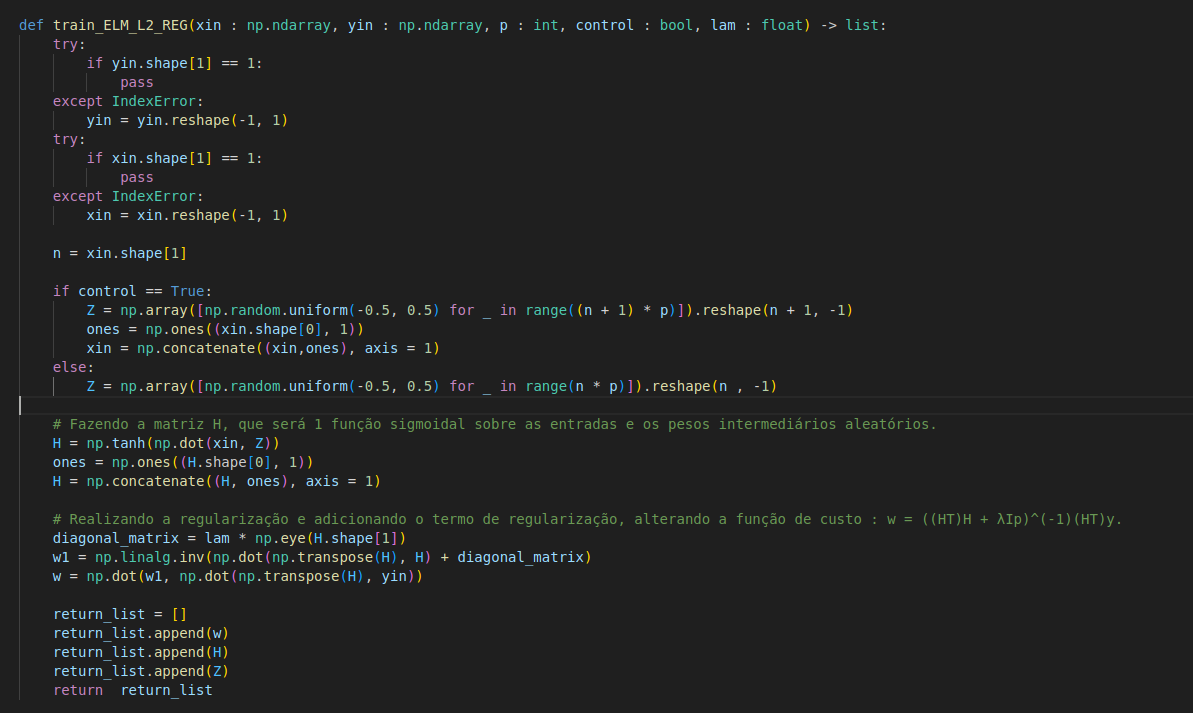
\includegraphics[height=3in]{train_L2.png}
    \caption{Função que implementa o treino das redes ELM com regularização L2.}
    \label{fig:example}
    
\end{figure}

\vspace{15pt}

No trabalho, um valor $\lambda$ que será somado a todos os elementos da diagonal principal no cálculo da pseudoinversa.


\vspace{20pt}

\subsection*{Pruning}

\vspace{20pt}

As técnicas de pruning consistem na remoção de parâmetros individuais ou neurônios inteiros de uma rede neural. Essa remoção segue uma heurística e um conjunto de regras que, quando executada corretamente provoca várias melhorias no modelo como : melhor generalização do modelo, menos gasto computacional, e uma singificante melhoria na velocidade de teste.[5]

\vspace{15pt}

Duas heurísticas serão utilizadas para a remoção dos parâmetros da rede. A primeira é a poda aleatória que consiste em escolher N pesos aleatórios e removê-los da rede, ou seja, alterar esses pesos aleatórios para o valor 0.  A segunda é a remoção dos parâmetros que tem menor influência na saída da rede, ou seja, os N menores pesos serão alterados para 0. Essa alteração dos parâmetros para 0 economiza recurso computacional na hora de realizar a validação do modelo, visto que menos cálculos precisarão ser realizados.

\begin{figure}[h]

    \centering
    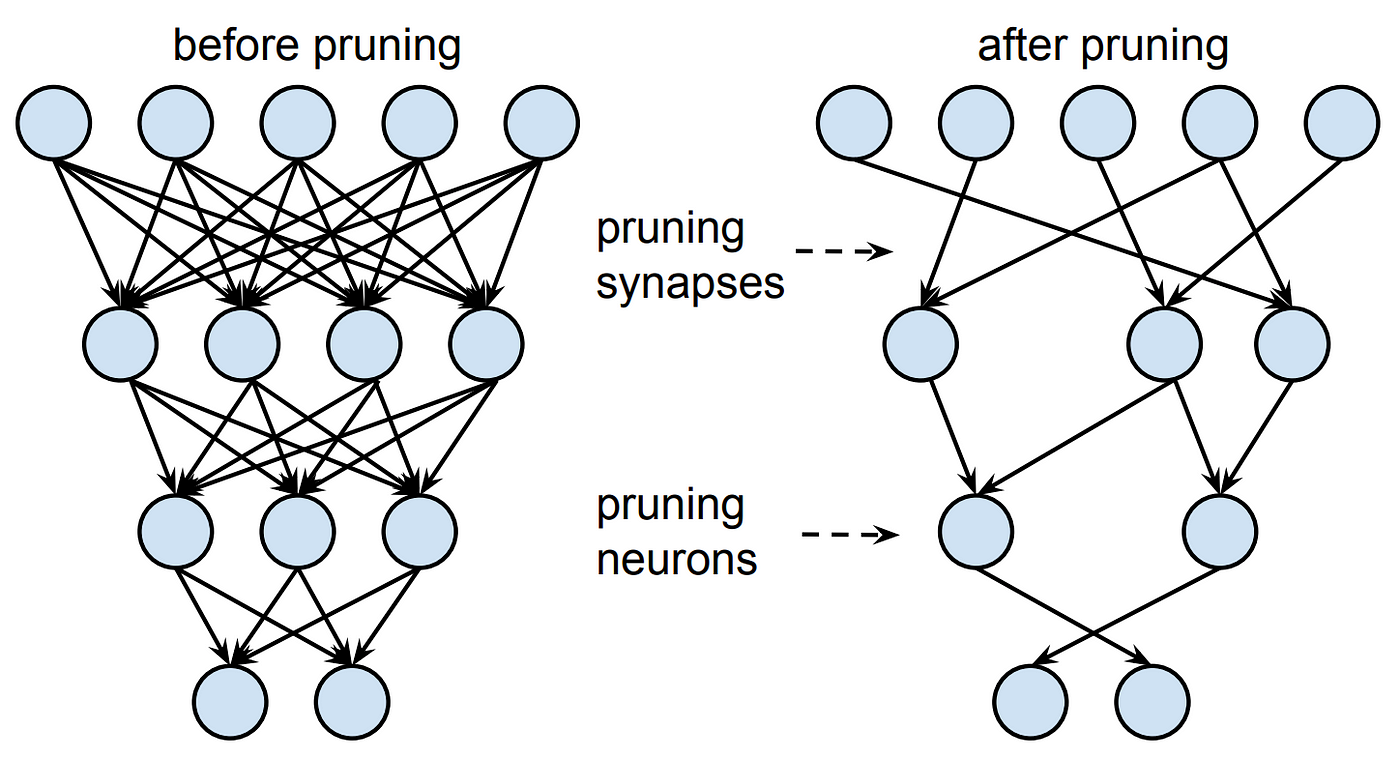
\includegraphics[height=2.5in]{n_net_after_before_pruning.png}
    \caption{Rede Neural antes e depois do pruning.}
    \label{fig:example}
    
\end{figure}

\newpage

\begin{figure}[h]

    \centering
    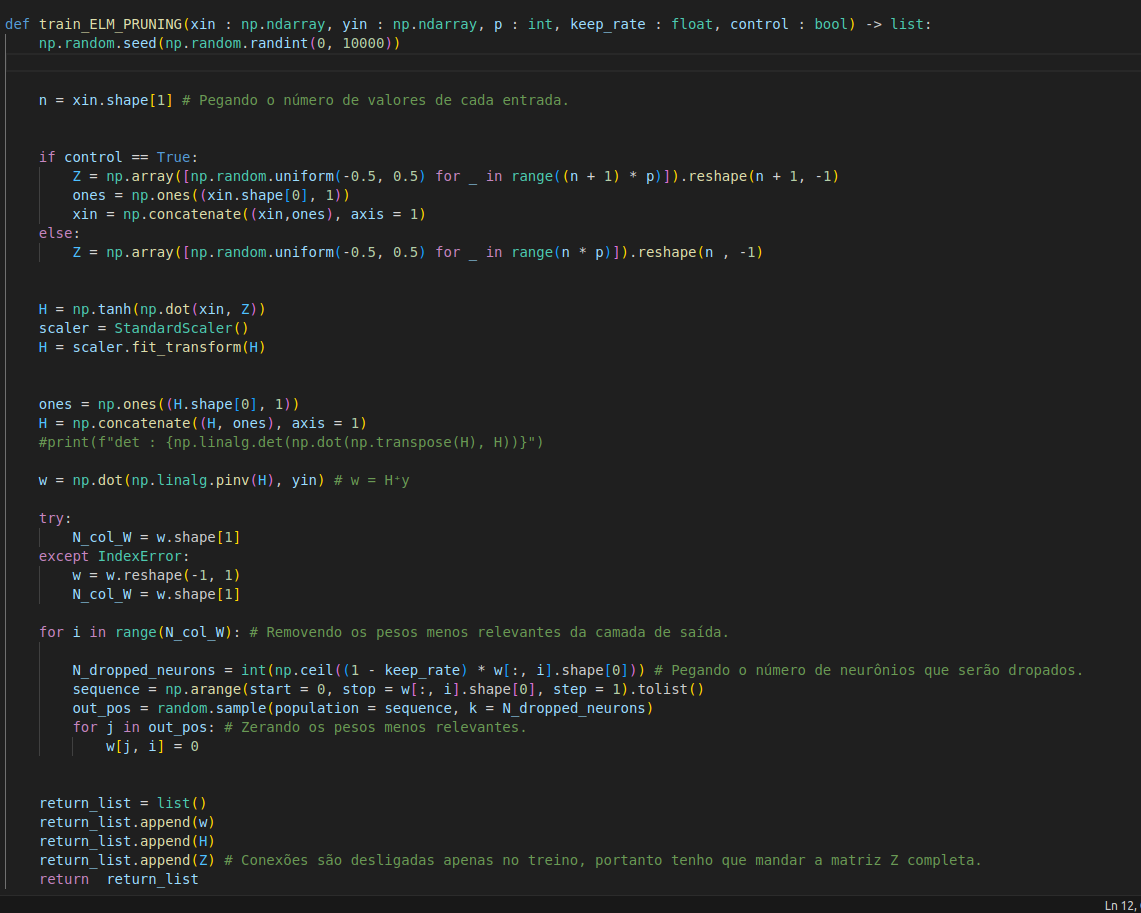
\includegraphics[height=3in]{random_prun.png}
    \caption{Função que implementa o treino das redes ELM com a poda aleatória.}
    \label{fig:example}
    
\end{figure}

\vspace{15pt}

\begin{figure}[h]

    \centering
    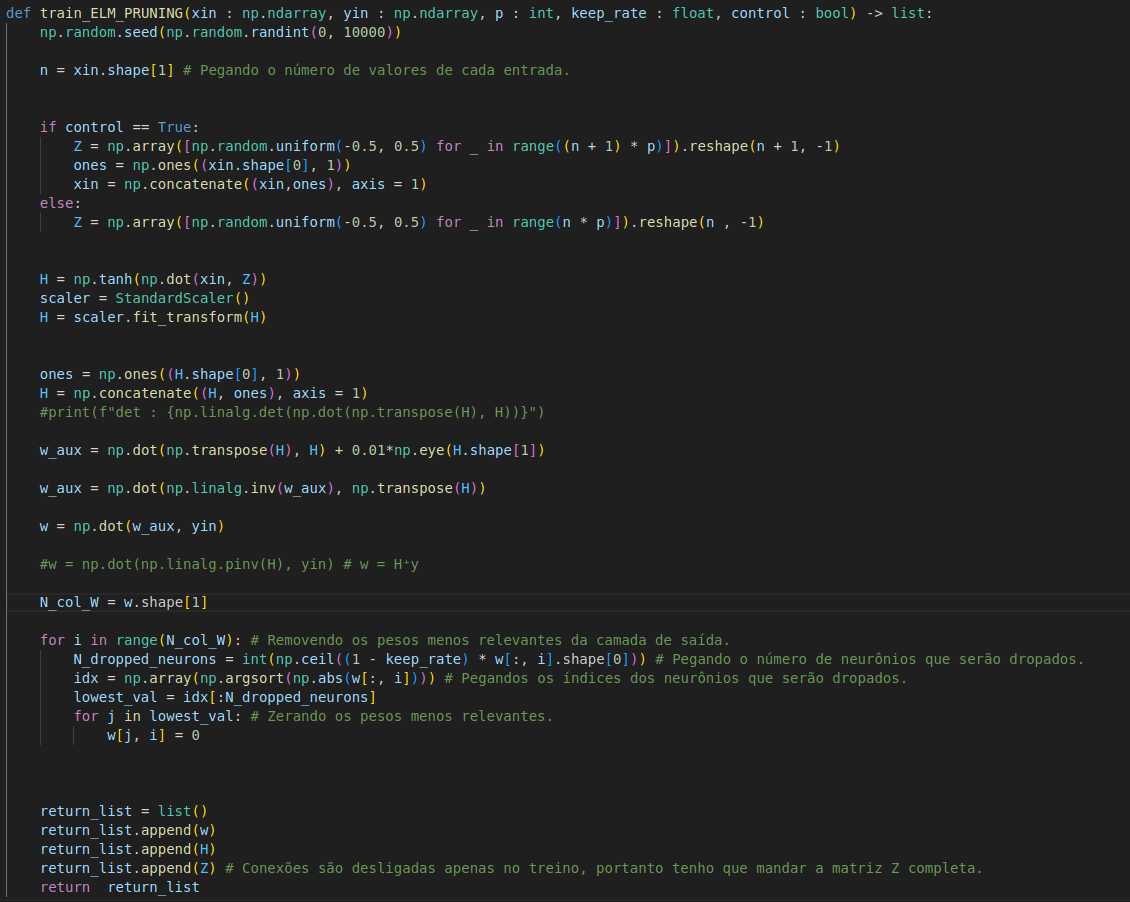
\includegraphics[height=3in]{prun_lowest_val.png}
    \caption{Função que implementa o treino das redes ELM com a poda do peso menos influente.}
    \label{fig:example}
    
\end{figure}

\vspace{15pt}

Portanto, ao utilizar os dois métodos de regularização, é de se esperar uma redução no termo variance do modelo (erro médio sobre os dados de teste), enquanto há um aumento no bias (erro médio nos dados de treino). Essa relação bias-variance indica um tradeoff entre o erro médio sobre os dados de treino e o erro médio sobre os dados de teste. Deixar o modelo bem regularizado e menos complexo reduz o termo variance enquanto aumenta o bias. Deixar o modelo pouco regularizado aumenta o termo variance e levará o modelo ao overfitting.

\newpage

\section*{Resultados e Discussões}

\vspace{15pt}

As imagens abaixo irão evidenciar a saída de cada um dos 3 modelos (Ridge Regression, Random Pruning, Pruning Lowest Value) para todos as bases de dados de classificação. O número de neurônios usados na camada intermediária em cada um dos modelos foi 100. Os valores de $\lambda$  e também do número de neurônios a serem cortados no pruning foram obtidos com o Grid Search Cross-Validation.

\vspace{15pt}

\subsection*{XOR}

\vspace{15pt}

\subsubsection*{Ridge Regression}

\vspace{15pt}

\begin{figure}[h]

    \centering
    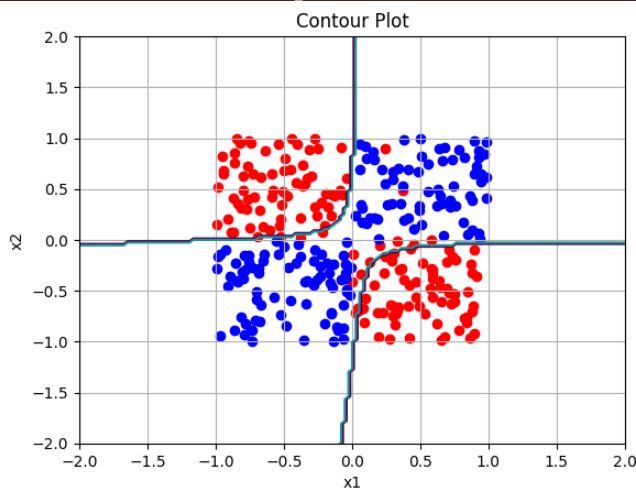
\includegraphics[height=2.3in]{Separation_L2.png}
    \caption{Gráfico de separação usando a regularização L2.}
    \label{fig:example}
    
\end{figure}

\vspace{15pt}

\begin{figure}[h]

    \centering
    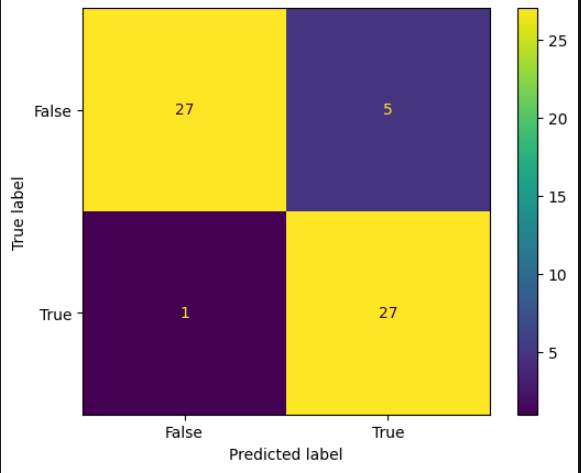
\includegraphics[height=2.3in]{Matrix_conf_XOR_L2.png}
    \caption{Matriz de confusão usando a regularização L2.}
    \label{fig:example}
    
\end{figure}


\newpage

\subsubsection*{Random Pruning}

\vspace{25pt}

\begin{figure}[h]

    \centering
    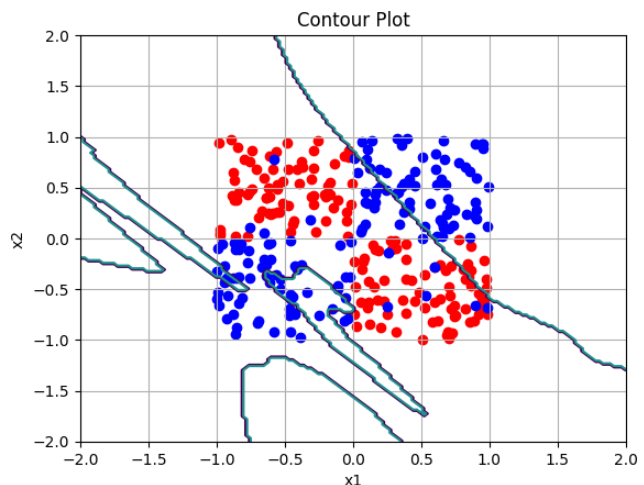
\includegraphics[height=3in]{sep_plot_random_pruning.png}
    \caption{Gráfico de separação usando o random pruning.}
    \label{fig:example}
    
\end{figure}

\vspace{25pt}

\begin{figure}[h]

    \centering
    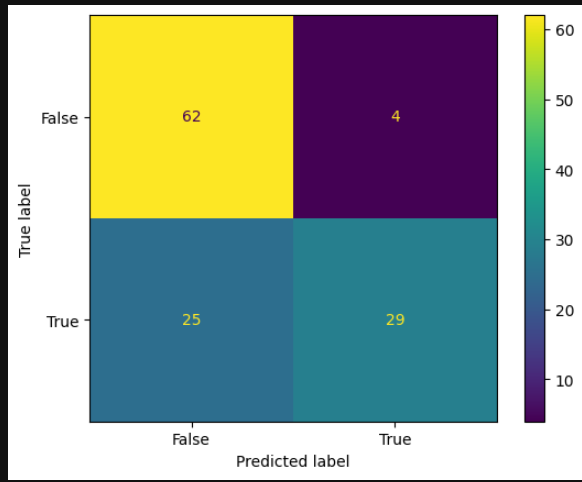
\includegraphics[height=3in]{conf_mat_random_pruning.png}
    \caption{Matriz de confusão usando o random pruning.}
    \label{fig:example}
    
\end{figure}

\newpage

\subsubsection*{Pruning Lowest Values}

\vspace{25pt}

\begin{figure}[h]

    \centering
    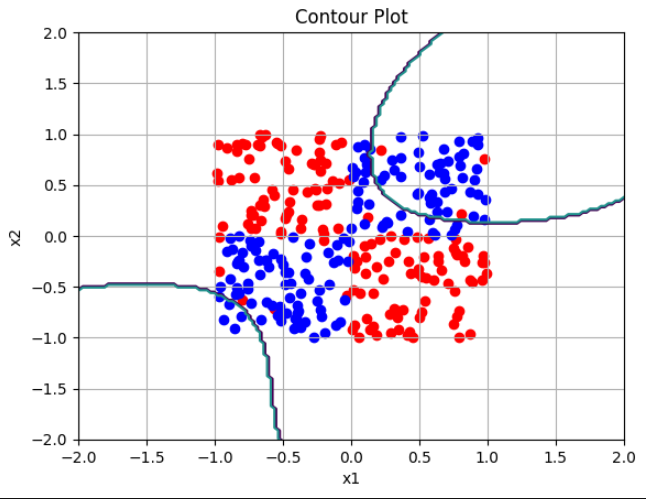
\includegraphics[height=3in]{plot_sep_prun_low_val.png}
    \caption{Gráfico de separação usando o pruning lowest value.}
    \label{fig:example}
    
\end{figure}

\vspace{25pt}

\begin{figure}[h]

    \centering
    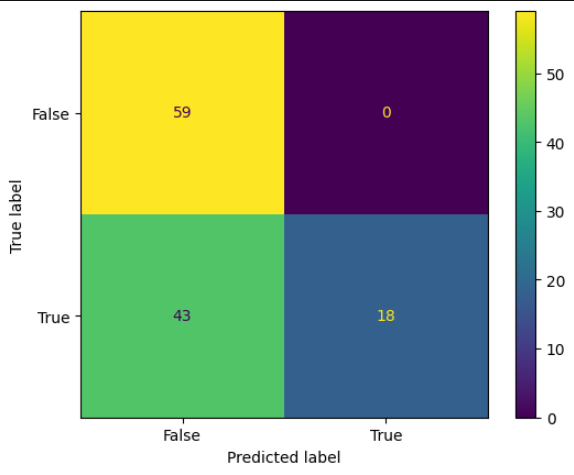
\includegraphics[height=3in]{conf_mat_prun_low_val.png}
    \caption{Matriz de confusão usando o pruning lowest value.}
    \label{fig:example}
    
\end{figure}

\newpage


\subsection*{Circle}

\vspace{15pt}

\subsubsection*{Ridge Regression}

\vspace{25pt}

\begin{figure}[h]

    \centering
    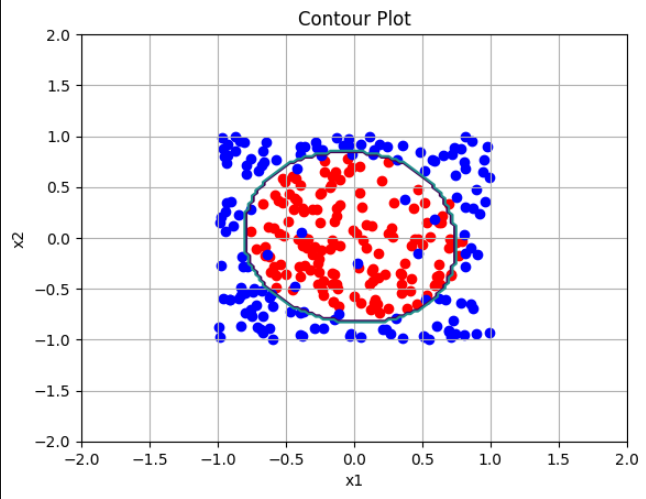
\includegraphics[height=3in]{sep_circle_l2.png}
    \caption{Gráfico de separação usando a regularização L2.}
    \label{fig:example}
    
\end{figure}

\vspace{25pt}

\begin{figure}[h]

    \centering
    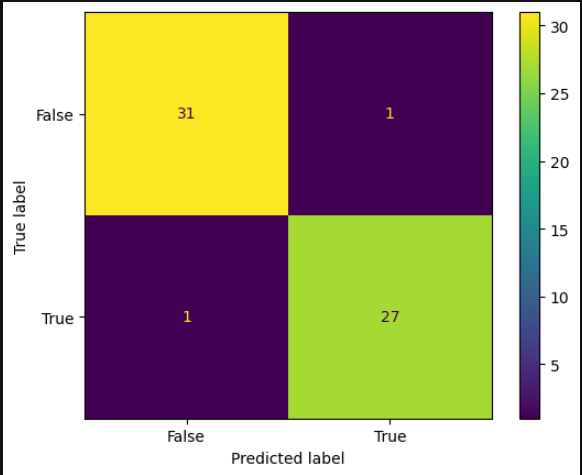
\includegraphics[height=3in]{conf_mat_circle_l2.png}
    \caption{Matriz de confusão usando a regularização L2.}
    \label{fig:example}
    
\end{figure}

\newpage

\subsubsection*{Random Pruning}

\vspace{25pt}

\begin{figure}[h]

    \centering
    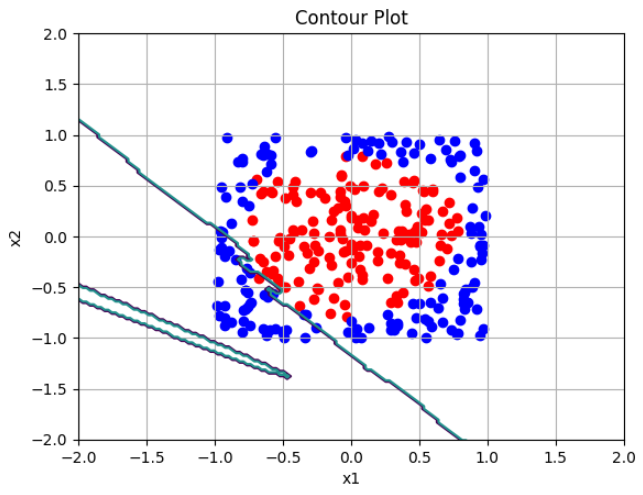
\includegraphics[height=3in]{sep_rp_circle.png}
    \caption{Gráfico de separação usando o random pruning.}
    \label{fig:example}
    
\end{figure}

\vspace{25pt}

\begin{figure}[h]

    \centering
    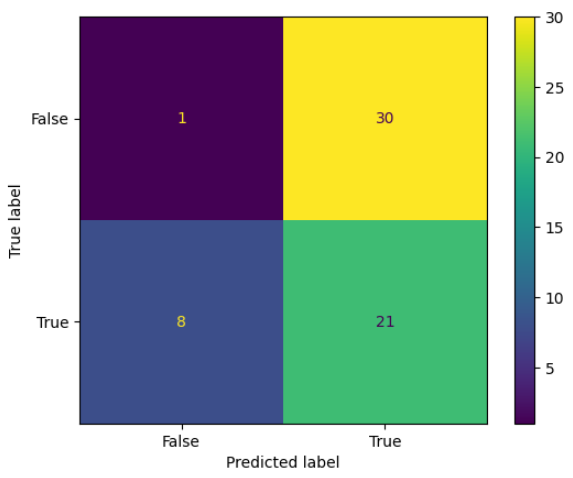
\includegraphics[height=3in]{conf_mat_rp_circle.png}
    \caption{Matriz de confusão usando o random pruning.}
    \label{fig:example}
    
\end{figure}

\newpage

\subsubsection*{Pruning Lowest Values}

\vspace{25pt}

\begin{figure}[h]

    \centering
    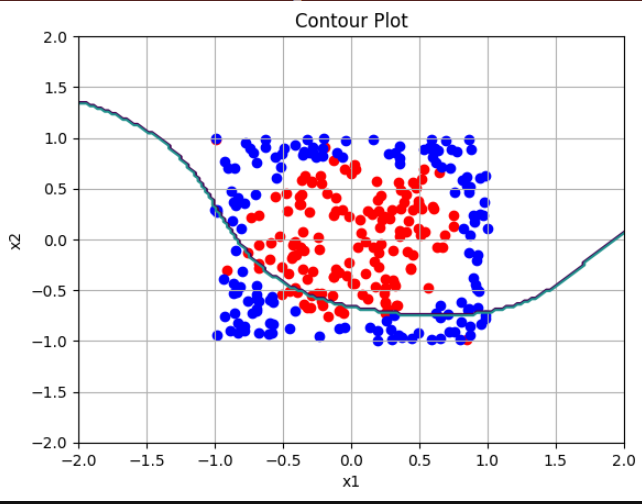
\includegraphics[height=3in]{sep_plv_circle.png}
    \caption{Gráfico de separação usando o pruning lowest value.}
    \label{fig:example}
    
\end{figure}

\vspace{25pt}

\begin{figure}[h]

    \centering
    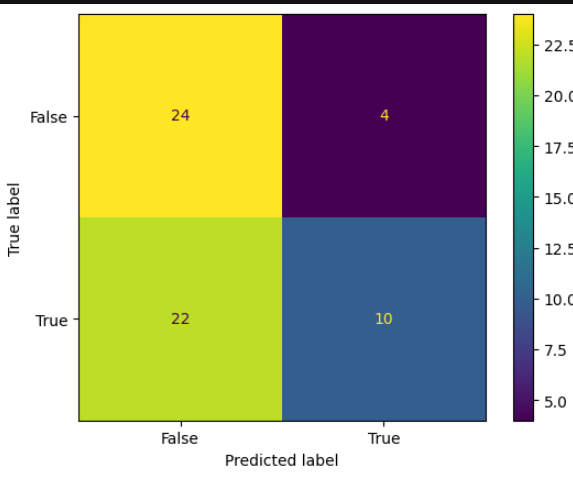
\includegraphics[height=3in]{conf_mat_plv.png}
    \caption{Matriz de confusão usando o pruning lowest value.}
    \label{fig:example}
    
\end{figure}

\newpage

\subsection*{Breast Cancer}

\vspace{15pt}

\subsubsection*{Ridge Regression}

\begin{figure}[h]

    \centering
    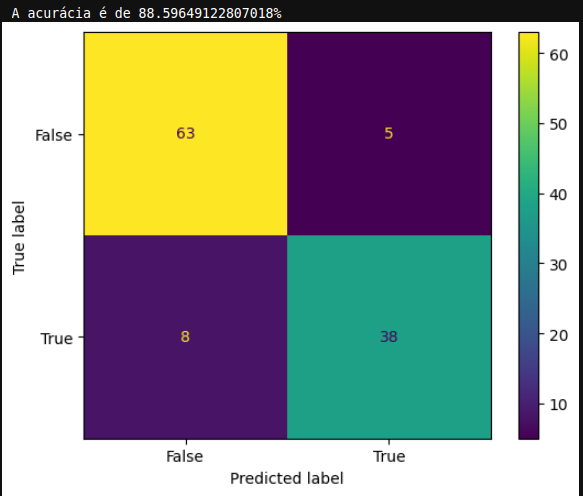
\includegraphics[height=2.5in]{conf_mat_bcancer_l2.png}
    \caption{Matriz de confusão na base de dados Breast Cancer usando o Ridge Regression.}
    \label{fig:example}
    
\end{figure}


\subsubsection*{Random Pruning}

\vspace{25pt}

\begin{figure}[h]

    \centering
    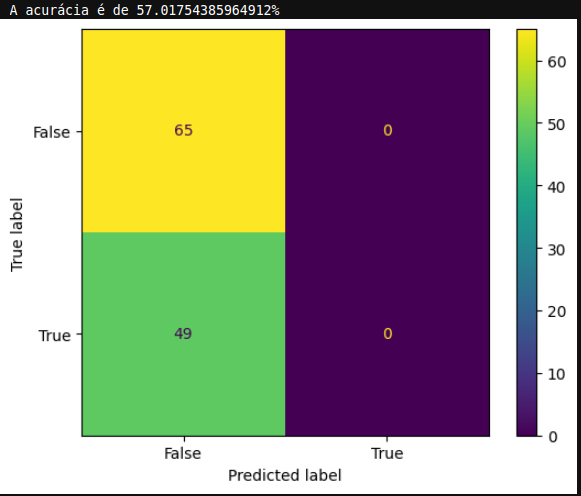
\includegraphics[height=2.5in]{conf_mat_random_pruning_bcancer.png}
    \caption{Matriz de confusão na base de dados Breast Cancer usando o random pruning.}
    \label{fig:example}
    
\end{figure}

\newpage

\subsubsection*{Pruning Lowest Values}

\begin{figure}[h]

    \centering
    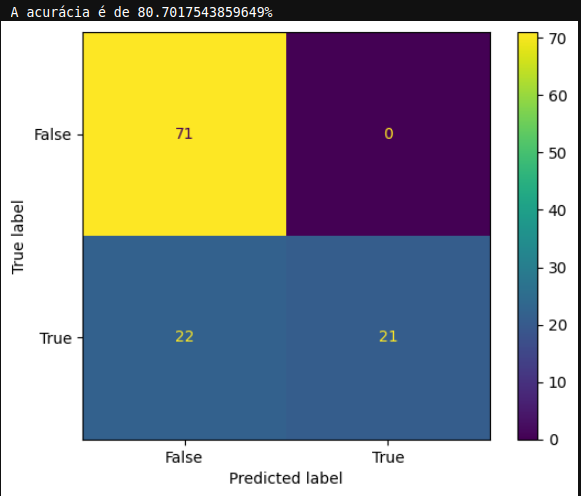
\includegraphics[height=2.5in]{conf_mat_plv_bcancer.png}
    \caption{Matriz de confusão na base de dados Breast Cancer usando o pruning lowest value.}
    \label{fig:example}
    
\end{figure}

\vspace{25pt}

Ao analisar as melhores situações para os 3 diferentes modelos com 100 neurônios na camada intermediária é possível concluir que o modelo com a regularização L2 contém as melhores acurácias e superfícies de separação. O modelo com a poda aleatória contém as piores superfícies de separação. O melhor valor de $\lambda$ foi variável em todas as bases de dados, com valores variando entre 0.2 e 0.7. O valor do Keep rate também foi variável, mas para um intervalo com valores maiores, indo de 0.7 ate 0.99. Isso indica que um número maior de pesos não nulos influencia consideravelmente a boa performance do modelo.

\vspace{25pt}

Ao reduzir o número de neurônios, pela metade e por um quarto, a acurácia e as superfícies de todos os 3 modelos também caem consideravelmente. O tempo de treinamento e teste também cai, pois o modelo fica menos complexo, necessitando realizar menos calculos computacionais.

\vspace{15pt}

Ao aumentar o número de neurônios, o treinamento e o teste demoram mais, e a acurácia aumenta um pouco.

\vspace{25pt}

Agora, iremos avaliar o desempenho dos 3 modelos para as bases de dados de regressão. Inicialmente uma função senoidal será aproximada, depois os modelos serão aplicados para as bases de dados Boston House e Wine Quality.

\newpage

\subsection{Aproximação senoidal}

\subsubsection*{Ridge Regression}

\vspace{25pt}

\begin{figure}[h]

    \centering
    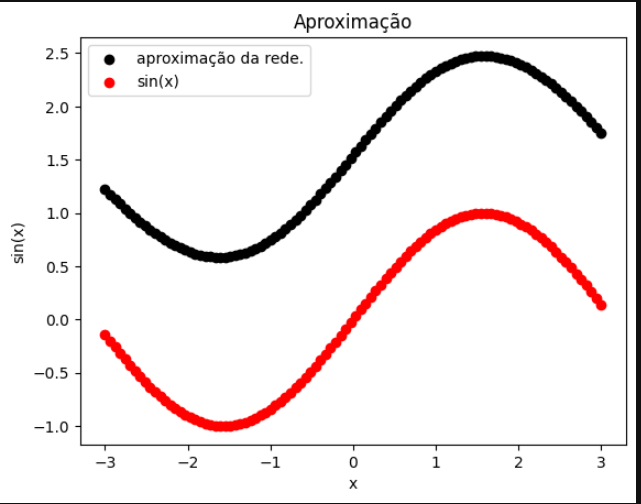
\includegraphics[height=2.5in]{sin_l2.png}
    \caption{Aproximação senoidal modelo com regularização L2.}
    \label{fig:example}
    
\end{figure}

\subsubsection*{Random Pruning}

\vspace{25pt}

\begin{figure}[h]

    \centering
    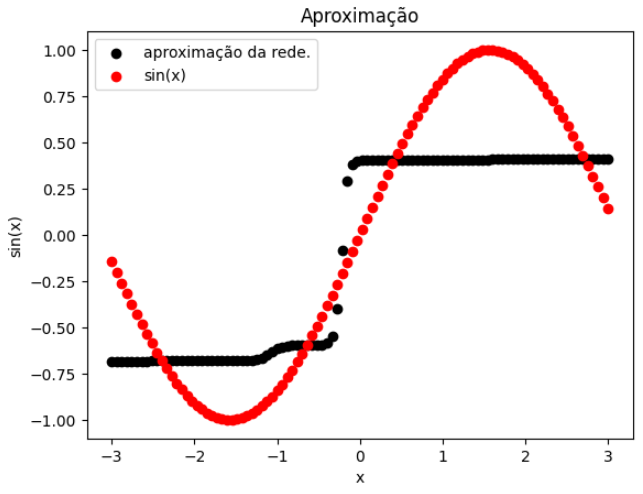
\includegraphics[height=2.5in]{sin_random_pru.png}
    \caption{Aproximação senoidal modelo com o random pruning.}
    \label{fig:example}
    
\end{figure}

\newpage

\subsubsection*{Pruning Lowest Values}

\vspace{25pt}

\begin{figure}[h]

    \centering
    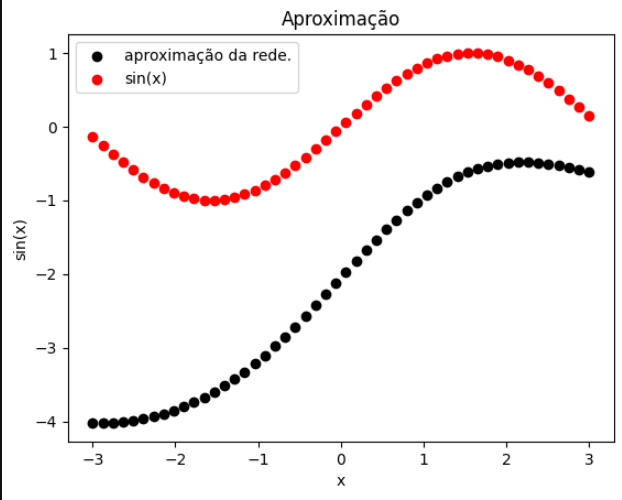
\includegraphics[height=2.5in]{sin_plv.png}
    \caption{Aproximação senoidal modelo com o pruning lowest value.}
    \label{fig:example}
    
\end{figure}










\subsection{Boston House}

\subsubsection*{Ridge Regression}

\vspace{25pt}

\begin{figure}[h]

    \centering
    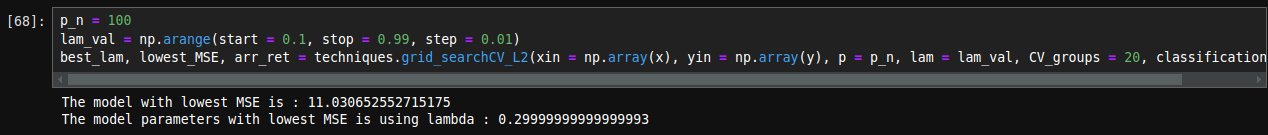
\includegraphics[height=0.75in]{MSE_l2_boston.png}
    \caption{MSE do modelo com regularização L2.}
    \label{fig:example}
    
\end{figure}

\subsubsection*{Random Pruning}

\vspace{25pt}

\begin{figure}[h]

    \centering
    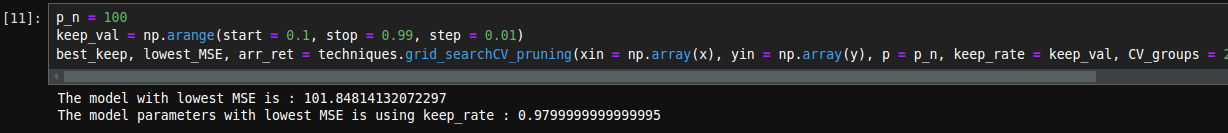
\includegraphics[height=0.75in]{MSE_random_prun_boston.png}
    \caption{MSE do modelo com o random pruning.}
    \label{fig:example}
    
\end{figure}

\newpage

\subsubsection*{Pruning Lowest Values}

\vspace{25pt}

\begin{figure}[h]

    \centering
    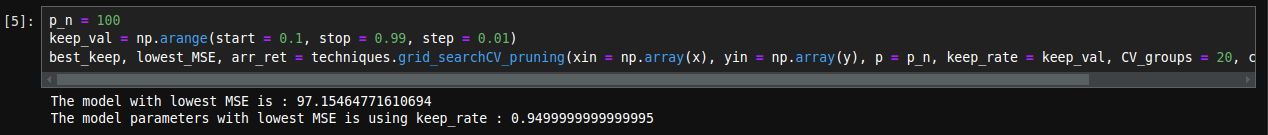
\includegraphics[height=0.75in]{MSE_prun_lv.png}
    \caption{MSE do modelo com o pruning lowest value.}
    \label{fig:example}
    
\end{figure}





\subsection{Wine Quality}

\subsubsection*{Ridge Regression}

\vspace{25pt}

\begin{figure}[h]

    \centering
    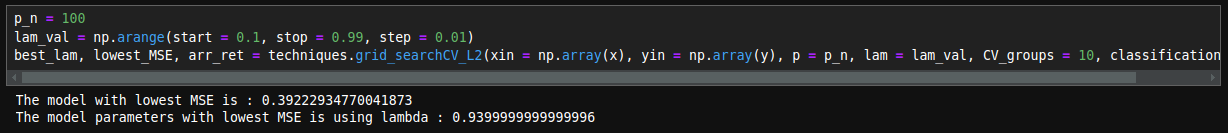
\includegraphics[height=0.75in]{MSE_L2_wine.png}
    \caption{MSE do modelo com regularização L2.}
    \label{fig:example}
    
\end{figure}

\subsubsection*{Random Pruning}

\vspace{25pt}

\begin{figure}[h]

    \centering
    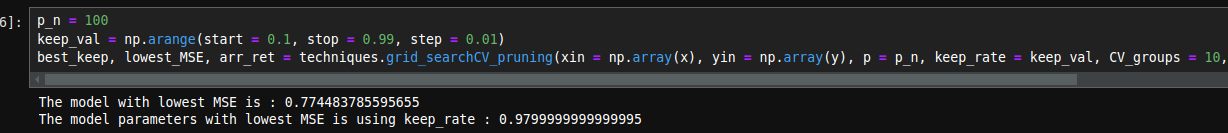
\includegraphics[height=0.75in]{MSE_random_prun.png}
    \caption{MSE do modelo com o random pruning.}
    \label{fig:example}
    
\end{figure}

\newpage

\subsubsection*{Pruning Lowest Values}

\vspace{25pt}

\begin{figure}[h]

    \centering
    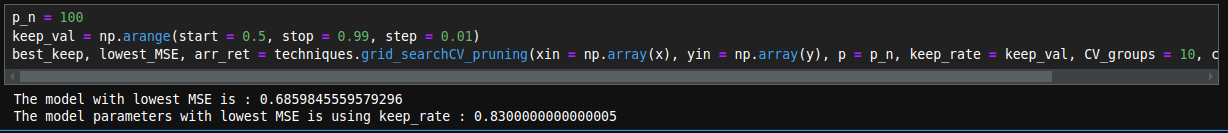
\includegraphics[height=0.75in]{MSE_plv.png}
    \caption{MSE do modelo com o pruning lowest value.}
    \label{fig:example}
    
\end{figure}

\vspace{25pt}

Portanto, fazendo uma análise sobre as aproximações, é podemos afirmar também que o modelo com regularização L2 também teve um melhor desempenho  e, para todos os casos, é o tipo de regularização que leva ao menor MSE. A poda aleatória é, visualmente, a pior aproximação para a função senoidal, enquanto a poda dos menores valores aproxima bem a curva senoidal.

\vspace{25pt}

\section*{Conclusão}

\vspace{20pt}

Após a realização de todos os treinamentos e testes para os diferentes modelos, é possível extrair conclusões significativas. Primeiramente, observa-se que o método de poda aleatória não se revela como o mais eficiente para realizar o pruning. Isso se deve ao fato de que pesos com maior influência na resposta podem ser inadvertidamente alterados para zero, impactando consideravelmente o resultado final do modelo. Por outro lado, a análise indica que o método de poda dos parâmetros menos influentes é uma abordagem viável. Ao adotar esse método, o modelo não tende a desenvolver viés e evita o overfitting, além de contribuir para a redução do tempo e do custo de teste. Além disso, observa-se que, em todas as instâncias, a aplicação da regularização Ridge Regression resultou em um desempenho superior para o modelo. Essa técnica demonstrou ser eficaz na mitigação de problemas de overfitting, contribuindo assim para a generalização e robustez do modelo.

\vspace{10pt}

Em suma, os resultados destacam a importância de escolher cuidadosamente o método de pruning e a regularização adequada para otimizar o desempenho e a eficiência dos modelos de aprendizado de máquina.

\newpage

\section*{Referências}

\vspace{20pt}

[1] HAYKIN, Simon. Neural Networks: a comprehensive foundation. 2. ed. India: Pearson Education, Inc, 2001.

\vspace{20pt}

[2] G. B. Huang, Q. Y. Zhu, and C. K. Siew, “Extreme learning machine: Theory and applications,” Neurocomputing, vol. 70, Dec. 2006.   

\vspace{20pt}

[3] Y. Miche, A. Sorjamaa, P. Bas, O. Simula, C. Jutten, and A. Lendasse, “OP-ELM: Optimally pruned extreme learning machine,” IEEE Trans. Neural Netw., vol. 21, no. 1, pp. 158–162, Jan. 2010.


\vspace{20pt}

[4] Braga, A P, Carvalho, A P L e Ludermir, T B (2007). Redes neurais artificiais: teoria e aplicações. LTC, Livros Técnicos e Científicos.

\vspace{20pt}

[5] CUN, Yann Le; DENKER, John S.; SOLLA, Sara A.. Optimal Brain Damage. Holmdel: Bell Laboratories, 1989.

\vspace{20pt}

[6] Canais confiáveis e renomados em plataformas como youtube.

\vspace{20pt}

[7] Sites como IBM, Microsoft, Google.

\end{document}

